\documentclass[10pt,a4paper]{article}
\usepackage[utf8]{inputenc}
\usepackage[T1]{fontenc}
\usepackage[spanish]{babel}
\usepackage{amsmath,amssymb}
\usepackage{graphicx}
\usepackage{float}
\usepackage{booktabs}
\usepackage{geometry}
\usepackage{listings}
\usepackage{xcolor}
\usepackage{hyperref}
\usepackage{caption}
\usepackage{setspace}
\usepackage{enumitem}
\usepackage{multirow}
\usepackage{csquotes}
\usepackage{titlesec}
\usepackage[style=apa,backend=biber,sorting=nyt]{biblatex}
\addbibresource{referencias.bib}

% --- Margenes segun pauta: 1.5cm sup, 1.5cm izq, 1.5cm der, 2cm inf ---
\geometry{top=1.5cm, left=1.5cm, right=1.5cm, bottom=2cm}

% --- Interlineado simple ---
\singlespacing

% --- Reducir espacios ---
\setlength{\parskip}{0pt}
\setlength{\parindent}{0pt}
\setlength{\abovedisplayskip}{3pt}
\setlength{\belowdisplayskip}{3pt}
\setlength{\abovedisplayshortskip}{2pt}
\setlength{\belowdisplayshortskip}{2pt}
\setlength{\textfloatsep}{4pt}
\setlength{\floatsep}{4pt}
\setlength{\intextsep}{4pt}

\captionsetup{labelfont=bf, labelsep=period, font=footnotesize, skip=1pt}
\addto\captionsspanish{%
  \renewcommand{\tablename}{Tabla}%
  \renewcommand{\figurename}{Fig.}%
}
\titlespacing*{\section}{0pt}{6pt}{3pt}
\titlespacing*{\subsection}{0pt}{4pt}{2pt}
\titlespacing*{\subsubsection}{0pt}{3pt}{1pt}

% --- Estilo de codigo R ---
\lstset{
  language=R,
  basicstyle=\ttfamily\footnotesize,
  backgroundcolor=\color{gray!8},
  frame=single,
  breaklines=true,
  keywordstyle=\color{blue!70!black},
  commentstyle=\color{green!50!black},
  stringstyle=\color{red!70!black},
  numbers=left,
  numberstyle=\tiny\color{gray},
  numbersep=5pt,
  xleftmargin=1.5em,
  framexleftmargin=1em
}

\hypersetup{colorlinks=true, linkcolor=blue!60!black, citecolor=blue!60!black, urlcolor=blue!60!black}

\pagestyle{plain}

\begin{document}

% =====================================================================
% 1) IDENTIFICACION
% =====================================================================
\begin{center}
  {\LARGE \textbf{Control 3: Agrupamiento K-Medias con R}} \\[4pt]
  {\normalsize Juan Mu\~noz, Vicente Rivera, Fernando Vald\'es} \\[2pt]
  {\small juan.munozveloso2023@alu.uct.cl, vrivera2023@alu.uct.cl, fvaldes2023@alu.uct.cl} \\[2pt]
  {\small Control 3, INFO1184, Semestre I-2026}
\end{center}

% =====================================================================
% 2) RESUMEN (100-130 palabras)
% =====================================================================
\section*{Resumen}

En este informe se analiza el algoritmo de agrupamiento k-medias aplicado a un conjunto de 7 observaciones bidimensionales $\mathbf{X} \in \mathbb{R}^2$. En la Pregunta 1 se desarrolla manualmente el algoritmo para $k=2$ durante 5 iteraciones, utilizando la distancia euclidiana y seleccionando $x_1$ y $x_2$ como centroides iniciales. Se verifica que las asignaciones se estabilizan en la iteraci\'on 2, por lo que las iteraciones restantes mantienen la misma partici\'on. En la Pregunta 2 se implementa el procedimiento en R para visualizar los datos y obtener agrupamientos con $k=2$ y $k=3$. Los resultados muestran una separaci\'on marcada entre $x_2$ y $x_4$, asociados a valores altos en $X_2$, y el resto del conjunto, confirmando la coherencia entre el an\'alisis manual y el computacional.

% =====================================================================
% 3) INTRODUCCION
% =====================================================================
\section{Introducci\'on}

El algoritmo k-medias es una t\'ecnica de aprendizaje no supervisado que particiona un conjunto de $n$ observaciones en $k$ grupos, buscando alta similitud intra-cluster y separaci\'on entre clusters. Dado un conjunto $\mathbf{X} = \{x_1, x_2, \ldots, x_n\}$ con $x_i \in \mathbb{R}^d$, el objetivo es encontrar una partici\'on $\mathcal{R} = \{R_1, R_2, \ldots, R_k\}$ y centroides $C = \{c_1, c_2, \ldots, c_k\}$ que minimicen la funci\'on objetivo
\begin{equation}
J(\mathcal{R}, C) = \sum_{j=1}^{k} \sum_{x \in R_j} \|x - c_j\|^2,
\label{eq:objetivo}
\end{equation}
la cual corresponde a la suma de cuadrados intra-cluster y, por tanto, a una medida de varianza interna de los grupos \parencite{duda2001}.

El procedimiento iterativo consiste en: (1) inicializar $k$ centroides, (2) asignar cada observaci\'on al centroide m\'as cercano seg\'un norma $L_2$, y (3) recalcular los centroides como la media de los puntos asignados; repitiendo estos pasos hasta convergencia \parencite{levano2026}. En cada iteraci\'on, el valor de la funci\'on objetivo en \eqref{eq:objetivo} no aumenta, lo que explica la convergencia del algoritmo a un punto fijo. Sin embargo, dicha convergencia no garantiza alcanzar el \'optimo global, ya que k-medias puede quedar atrapado en \'optimos locales dependiendo de la configuraci\'on inicial de los centroides.

Por esta raz\'on, la inicializaci\'on de centroides es un aspecto cr\'itico: distintas elecciones iniciales pueden generar trayectorias de reasignaci\'on diferentes, alterar el n\'umero de iteraciones e incluso conducir a particiones finales distintas. En implementaciones computacionales, esta sensibilidad suele mitigarse mediante m\'ultiples arranques y la selecci\'on de la soluci\'on con menor valor de la funci\'on objetivo. De manera complementaria, la elecci\'on de $k$ puede apoyarse en criterios exploratorios como el m\'etodo del codo, que compara c\'omo disminuye la dispersi\'on intra-cluster al aumentar el n\'umero de grupos.

En este trabajo se aplica k-medias al conjunto fijo $\mathbf{X} = \{(1.5, -1.88),\ (26.5, 100.55),\ (-1.5, -6.66),\ (29.7, 89.66),\ (3.1416, 2.7181),\ (8.8, -7.5),\ (-8.11, -7.56)\}$, primero de forma manual (Pregunta 1) y luego computacionalmente en R (Pregunta 2). El objetivo es resolver ordenadamente el desarrollo solicitado, contrastar la teor\'ia con los resultados obtenidos y justificar la interpretaci\'on de los agrupamientos. Para mantener la notaci\'on ordenada, en la resoluci\'on manual se denotan las asignaciones iterativas como $G_j^{(t)}$, mientras que en la implementaci\'on computacional las particiones finales se representan como $R_j$ para un valor fijo de $k$.

% =====================================================================
% 4) DESARROLLO
% =====================================================================
\section{Desarrollo}

\subsection{Pregunta 1: K-medias manual ($k=2$, 5 iteraciones)}

Se aplica el algoritmo k-medias con $k=2$ y norma $L_2$, usando la distancia euclidiana
\begin{equation}
d(x_i, C_j) = \sqrt{(x_{i1} - c_{j1})^2 + (x_{i2} - c_{j2})^2}.
\label{eq:distancia}
\end{equation}
Como el enunciado no fija centroides iniciales, se seleccionan las dos primeras observaciones como criterio simple, expl\'icito y reproducible para el desarrollo manual:
\begin{equation}
C_1^{(0)} = x_1 = (1.5,\; -1.88), \qquad C_2^{(0)} = x_2 = (26.5,\; 100.55)
\label{eq:centroides-iniciales}
\end{equation}

\subsubsection*{S\'intesis del desarrollo}

Siguiendo la pauta del control, el procedimiento manual completo se realiz\'o iteraci\'on por iteraci\'on. En el cuerpo principal se presenta una s\'intesis de resultados y en el \textbf{Anexo A.1} se conserva el detalle exhaustivo de distancias, reasignaciones y rec\'alculo de centroides.

C\'alculos representativos:
\begin{align}
d(x_3, C_1) &= \sqrt{(-1.5-1.5)^2 + (-6.66+1.88)^2} = \sqrt{9 + 22.85} = 5.64 \label{eq:calc-x3}\\
d(x_4, C_2) &= \sqrt{(29.7-26.5)^2 + (89.66-100.55)^2} = \sqrt{10.24 + 118.59} = 11.35 \label{eq:calc-x4}
\end{align}

\begin{align}
C_1^{(1)} &= \frac{1}{5}(1.5 + (-1.5) + 3.1416 + 8.8 + (-8.11),\; -1.88 + (-6.66) + 2.7181 + (-7.5) + (-7.56)) \notag\\
&= \left(\frac{3.8316}{5},\; \frac{-20.8819}{5}\right) = (0.76632,\; -4.17638) \label{eq:centroide-c1}\\[4pt]
C_2^{(1)} &= \frac{1}{2}(26.5 + 29.7,\; 100.55 + 89.66) = (28.1,\; 95.105) \label{eq:centroide-c2}
\end{align}

\begin{table}[H]
\centering
\scriptsize
\begin{tabular}{p{1.5cm} p{5.8cm} p{5.2cm} p{2.7cm}}
\toprule
\textbf{Iter.} & \textbf{Asignaciones} & \textbf{Centroides} & \textbf{Estado} \\
\midrule
1 & $G_1^{(1)}=\{x_1,x_3,x_5,x_6,x_7\}$; $G_2^{(1)}=\{x_2,x_4\}$ & $C_1^{(1)}=(0.76632,-4.17638)$; $C_2^{(1)}=(28.1,95.105)$ & Reasignaci\'on inicial \\
2 & $G_1^{(2)}=\{x_1,x_3,x_5,x_6,x_7\}$; $G_2^{(2)}=\{x_2,x_4\}$ & $C_1^{(2)}=(0.76632,-4.17638)$; $C_2^{(2)}=(28.1,95.105)$ & Convergencia \\
3--5 & Id\'enticas a la iteraci\'on 2 & Id\'enticos a la iteraci\'on 2 & Sin cambios \\
\bottomrule
\end{tabular}
\caption{S\'intesis del desarrollo manual de k-medias para $k=2$.}
\label{tab:manual-resumen}
\end{table}

La Tabla~\ref{tab:manual-resumen} muestra que las asignaciones de la iteraci\'on 2 coinciden con las de la iteraci\'on 1 y que los centroides permanecen estables desde ese momento. El algoritmo separa naturalmente los datos en un grupo de puntos cercanos a la zona baja del plano ($G_1$) y otro formado por los dos puntos con valores elevados en $X_2$ ($G_2$). La convergencia r\'apida se explica por dos factores complementarios: la brecha de m\'as de 86 unidades en la segunda componente entre ambos grupos y la inicializaci\'on elegida en \eqref{eq:centroides-iniciales}, que ubica desde el comienzo un centroide en la regi\'on inferior y otro en la regi\'on superior. En consecuencia, el n\'umero de reasignaciones posibles es bajo y la funci\'on objetivo de \eqref{eq:objetivo} se estabiliza tempranamente. El desarrollo manual completo, iteraci\'on por iteraci\'on, se presenta en el \textbf{Anexo A.1}.

% =====================================================================
\subsection{Pregunta 2: Implementaci\'on en R}

\textbf{a) Gr\'afico de dispersi\'on:} Se ingresan las 7 observaciones bidimensionales en un \texttt{data.frame} y se genera un gr\'afico de dispersi\'on con \texttt{plot()}, etiquetando cada punto $x_i$. La Fig.~\ref{fig:dispersion}, ubicada en el Anexo, muestra la distribuci\'on espacial de los datos, donde se observa que $x_2(26.5, 100.55)$ y $x_4(29.7, 89.66)$ est\'an alejados del resto, sugiriendo una estructura natural de al menos 2 clusters.

\textbf{b) y c) K-medias con $k=2$ y $k=3$:} Se aplica \texttt{kmeans(datos, centers=k, nstart=25)} con \texttt{set.seed(42)} para reproducibilidad. El par\'ametro \texttt{nstart=25} es pertinente en este contexto porque k-medias es sensible a la inicializaci\'on y puede converger a soluciones locales distintas. Conforme a la pauta general, el script completo se presenta exclusivamente en el \textbf{Anexo A.2}. La Tabla~\ref{tab:resultados-r} resume simult\'aneamente las particiones obtenidas y los centroides estimados.

\begin{table}[H]
\centering
\scriptsize
\begin{tabular}{@{}p{0.9cm} p{1.1cm} p{8.7cm} p{3.2cm}@{}}
\toprule
\textbf{k} & \textbf{Cluster} & \textbf{Elementos} & \textbf{Centroide} \\
\midrule
\multirow{2}{*}{2} & $R_1$ & $x_1(1.5, -1.88)$, $x_3(-1.5, -6.66)$, $x_5(3.14, 2.72)$, $x_6(8.8, -7.5)$, $x_7(-8.11, -7.56)$ & $(0.7663, -4.1764)$ \\
& $R_2$ & $x_2(26.5, 100.55)$, $x_4(29.7, 89.66)$ & $(28.1000, 95.1050)$ \\
\midrule
\multirow{3}{*}{3} & $R_1$ & $x_1(1.5, -1.88)$, $x_5(3.14, 2.72)$, $x_6(8.8, -7.5)$ & $(4.4805, -2.2206)$ \\
& $R_2$ & $x_2(26.5, 100.55)$, $x_4(29.7, 89.66)$ & $(28.1000, 95.1050)$ \\
& $R_3$ & $x_3(-1.5, -6.66)$, $x_7(-8.11, -7.56)$ & $(-4.8050, -7.1100)$ \\
\bottomrule
\end{tabular}
\caption{Resultados de k-medias para $k=2$ y $k=3$. Se verifica $R_i \neq \varnothing$, $\bigcup_i R_i = \mathbf{X}$ y $R_i \cap R_j = \varnothing$ para $i \neq j$.}
\label{tab:resultados-r}
\end{table}

La Tabla~\ref{tab:resultados-r} resume las particiones obtenidas y sus centroides. En ambos casos, $x_2$ y $x_4$ forman un cluster diferenciado por sus valores elevados en $X_2$ (100.55 y 89.66, respectivamente). Con $k=3$, el cluster inferior se subdivide en un subconjunto de puntos centrales ($x_1, x_5, x_6$) y otro de puntos con coordenadas predominantemente negativas ($x_3, x_7$). Esta partici\'on es coherente con la geometr\'ia observada en la Fig.~\ref{fig:dispersion}: el agrupamiento superior permanece estable, mientras que la variaci\'on adicional se concentra en la regi\'on inferior del plano. Los centros se marcan con una cruz ($\times$) en las Fig.~\ref{fig:k2} y~\ref{fig:k3}, y el centroide del cluster superior se mantiene en $(28.10, 95.11)$ para ambos valores de $k$, lo cual confirma la estabilidad de dicho agrupamiento. Adem\'as, los resultados de R coinciden exactamente con los obtenidos manualmente en la Pregunta 1 para $k=2$, validando ambos procedimientos. A partir de estos resultados, es razonable inferir que otras inicializaciones podr\'ian modificar la subdivisi\'on del grupo inferior, especialmente cuando $k=3$, pero tendr\'ian un efecto limitado sobre el cluster superior dada su marcada separaci\'on respecto del resto de los datos.

% =====================================================================
% 5) REFLEXION
% =====================================================================
\section{Reflexi\'on}

Este control permiti\'o contrastar la teor\'ia de k-medias con resultados manuales y computacionales consistentes. La convergencia en la iteraci\'on 2 es coherente con la minimizaci\'on de la varianza intra-cluster y se explica por la fuerte separaci\'on del par $\{x_2, x_4\}$ respecto del resto, especialmente en la componente $X_2$. Por ello, la reasignaci\'on de observaciones es m\'inima y la funci\'on objetivo se estabiliza r\'apidamente.

La comparaci\'on entre $k=2$ y $k=3$ muestra que la elecci\'on de $k$ modifica la granularidad del an\'alisis. Con $k=2$ se obtiene la estructura dominante del conjunto; con $k=3$ se preserva el cluster superior y se refina la regi\'on inferior. Adem\'as, otras inicializaciones podr\'ian alterar la subdivisi\'on inferior o aumentar el n\'umero de iteraciones, lo que justifica el uso de \texttt{nstart=25}. Si se quisiera formalizar la selecci\'on de $k$, una extensi\'on natural del trabajo ser\'ia aplicar el m\'etodo del codo.

\section{Conclusiones}

\textbf{Juan Mu\~noz:} El desarrollo manual confirma que $k=2$ representa adecuadamente la estructura principal del conjunto, ya que la separaci\'on del grupo superior $\{x_2, x_4\}$ se mantiene estable desde la iteraci\'on 2.

\textbf{Vicente Rivera:} La implementaci\'on en R valid\'o exactamente los resultados manuales para $k=2$ y mostr\'o que la reproducibilidad y los m\'ultiples arranques son relevantes debido a la sensibilidad de k-medias a la inicializaci\'on.

\textbf{Fernando Vald\'es:} La comparaci\'on entre $k=2$ y $k=3$ evidencia que aumentar el n\'umero de clusters permite refinar la regi\'on inferior sin alterar el grupo superior, por lo que la elecci\'on de $k$ debe responder al objetivo del an\'alisis.

% =====================================================================
% 6) REFERENCIAS (APA, solo dos)
% =====================================================================
\section*{Referencias}
\printbibliography[heading=none]

% =====================================================================
% 7) ANEXO
% =====================================================================
\newpage
\section*{Anexo}

\subsection*{A.1 Desarrollo manual de la Pregunta 1}

En esta secci\'on se presenta el desarrollo manual, ordenado y paso a paso, del algoritmo k-medias con $k=2$ y norma $L_2$, para las 5 iteraciones solicitadas.

\begin{figure}[H]
  \centering
  \includegraphics[width=0.85\textwidth]{Imagenprocedimiento1.jpg}
  \caption{Iteraci\'on 1: datos y f\'ormulas utilizadas en el problema.}
\end{figure}

\begin{figure}[H]
  \centering
  \includegraphics[width=0.85\textwidth]{Imagenprocedimiento2.jpg}
  \caption{C\'alculo de la iteraci\'on 1 y obtenci\'on de la primera asignaci\'on.}
\end{figure}

\begin{figure}[H]
  \centering
  \includegraphics[width=0.85\textwidth]{Imagenprocedimiento3.jpg}
  \caption{Rec\'alculo de los centroides para la iteraci\'on 2.}
\end{figure}

\begin{figure}[H]
  \centering
  \includegraphics[width=0.85\textwidth]{Imagenprocedimiento4.jpg}
  \caption{C\'alculo de la iteraci\'on 2 con centroides actualizados.}
\end{figure}

\begin{figure}[H]
  \centering
  \includegraphics[width=0.85\textwidth]{Imagenprocedimiento5.jpg}
  \caption{C\'alculo de las iteraciones 3, 4 y 5 con resultados estabilizados.}
\end{figure}

\subsection*{A.2 Script R completo (Pregunta 2)}

\begin{lstlisting}
# ============================================================
# Control 3 - INFO1184 - Pregunta 2
# K-Medias con R
# ============================================================

# --- Datos X en R^2, i=7 ---
datos <- data.frame(
  X1 = c(1.5, 26.5, -1.5, 29.7, 3.1416, 8.8, -8.11),
  X2 = c(-1.88, 100.55, -6.66, 89.66, 2.7181, -7.5, -7.56)
)
rownames(datos) <- paste0("x", 1:7)

# --- a) Grafico de dispersion ---
plot(datos$X1, datos$X2,
     main = "Dispersion de los datos X",
     xlab = expression(X[1]), ylab = expression(X[2]),
     pch = 19, col = "black", cex = 1.3)
text(datos$X1, datos$X2, labels = rownames(datos),
     pos = 4, cex = 0.8)
grid()

# --- b) K-medias k=2 ---
set.seed(42)
km2 <- kmeans(datos, centers = 2, nstart = 25)
colores_k2 <- c("red", "blue")
plot(datos$X1, datos$X2,
     main = "K-Medias con k=2",
     xlab = expression(X[1]), ylab = expression(X[2]),
     pch = 19, col = colores_k2[km2$cluster], cex = 1.3)
text(datos$X1, datos$X2, labels = rownames(datos),
     pos = 4, cex = 0.8)
points(km2$centers[,1], km2$centers[,2],
       pch = 4, col = colores_k2, cex = 2.5, lwd = 3)
legend("topleft", legend = paste("Cluster", 1:2),
       col = colores_k2, pch = 19, cex = 0.7)
grid()

# --- K-medias k=3 ---
set.seed(42)
km3 <- kmeans(datos, centers = 3, nstart = 25)
colores_k3 <- c("red", "blue", "darkgreen")
plot(datos$X1, datos$X2,
     main = "K-Medias con k=3",
     xlab = expression(X[1]), ylab = expression(X[2]),
     pch = 19, col = colores_k3[km3$cluster], cex = 1.3)
text(datos$X1, datos$X2, labels = rownames(datos),
     pos = 4, cex = 0.8)
points(km3$centers[,1], km3$centers[,2],
       pch = 4, col = colores_k3, cex = 2.5, lwd = 3)
legend("topleft", legend = paste("Cluster", 1:3),
       col = colores_k3, pch = 19, cex = 0.7)
grid()

# --- c) Imprimir centros ---
cat("Centros k=2:\n"); print(km2$centers)
cat("Centros k=3:\n"); print(km3$centers)
\end{lstlisting}

\subsection*{A.3 Figuras generadas}

\begin{figure}[H]
  \centering
  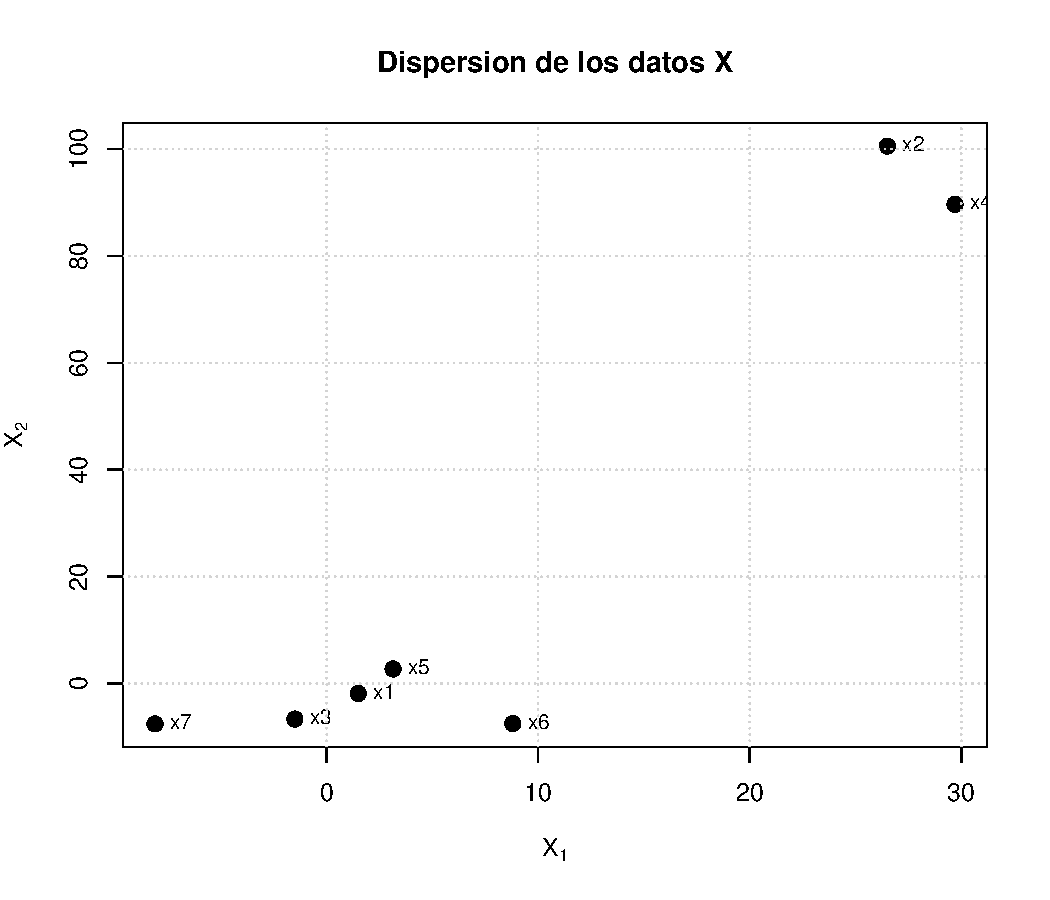
\includegraphics[width=0.75\textwidth]{dispersion.pdf}
  \caption{Gr\'afico de dispersi\'on de los 7 puntos $\mathbf{X} \in \mathbb{R}^2$.}
  \label{fig:dispersion}
\end{figure}

\begin{figure}[H]
  \centering
  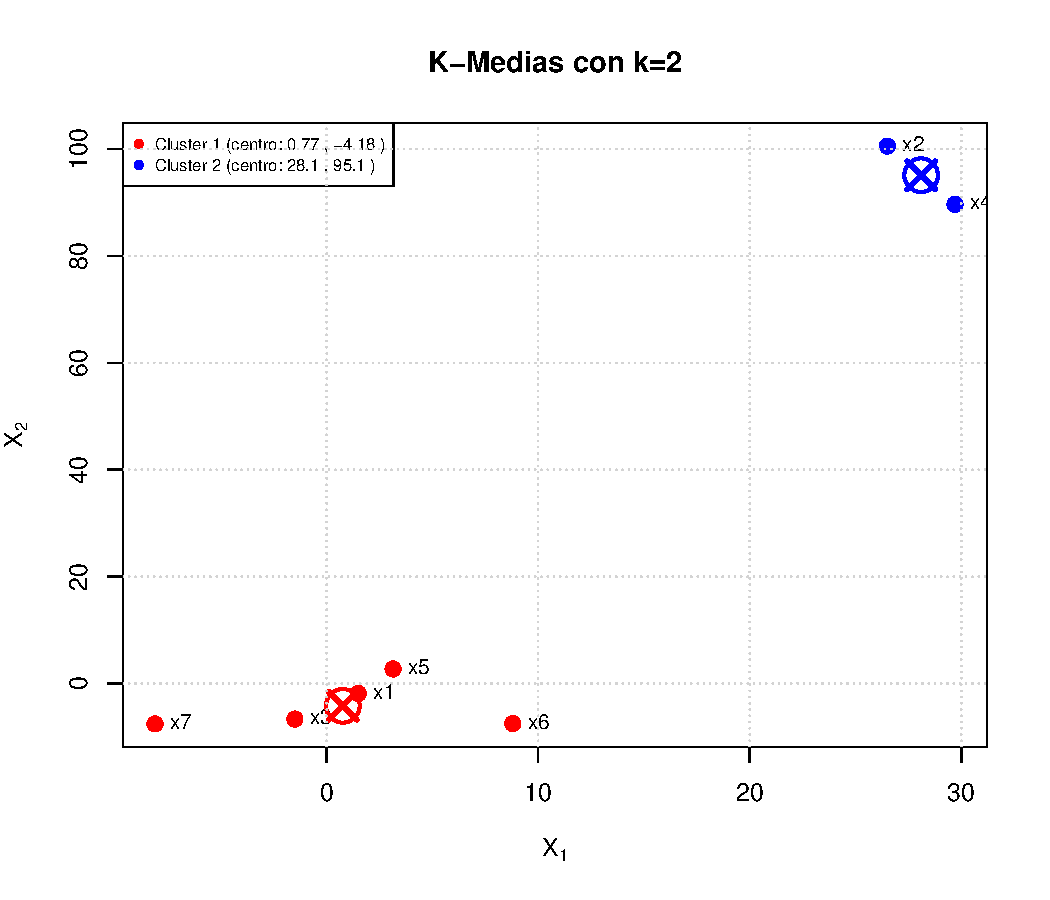
\includegraphics[width=0.75\textwidth]{kmeans_k2.pdf}
  \caption{K-medias con $k=2$. Los centros se marcan con $\times$.}
  \label{fig:k2}
\end{figure}

\begin{figure}[H]
  \centering
  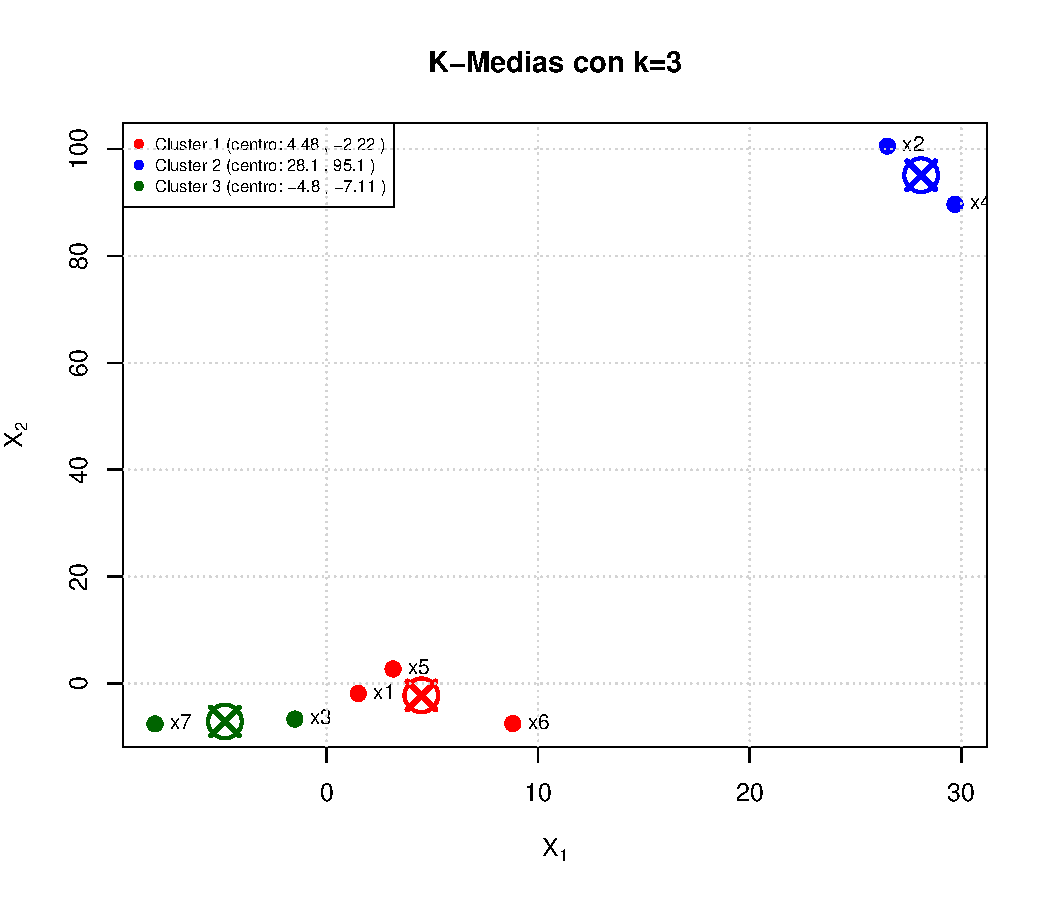
\includegraphics[width=0.75\textwidth]{kmeans_k3.pdf}
  \caption{K-medias con $k=3$. Los centros se marcan con $\times$.}
  \label{fig:k3}
\end{figure}

\subsection*{A.4 Bit\'acora de trabajo}

\begin{table}[H]
\centering
\footnotesize
\begin{tabular}{p{2.5cm} p{3cm} p{8cm}}
\toprule
\textbf{Fecha} & \textbf{Actividad} & \textbf{Descripci\'on} \\
\midrule
15/04/2026 & Lectura del enunciado & Comprensi\'on del problema y revisi\'on de diapositivas sobre datos conglomerados (semana 3). \\
15/04/2026 & Desarrollo Pregunta 1 & C\'alculos manuales de k-medias $k=2$, 5 iteraciones con norma $L_2$. \\
15/04/2026 & Desarrollo Pregunta 2 & Implementaci\'on del script R: dispersi\'on, k-medias $k=2$ y $k=3$, centroides. \\
15/04/2026 & Redacci\'on del informe & Elaboraci\'on del informe en \LaTeX{} seg\'un la pauta, integraci\'on de figuras, reflexi\'on y conclusiones. \\
\bottomrule
\end{tabular}
\caption{Bit\'acora de actividades del control.}
\end{table}

\end{document}
